\chapter{ENTWURF}
\label{sec:security_analyse}

\section{ANFORDERUNGEN}
\label{sec:Threat_model}
Das primäre Designziel dieses Entwurfs ist es, die Laufzeit des Algorithmus so weit wie möglich zu minimieren und den Hardwareaufwand so gering wie möglich zu halten. In der Praxis benötigt der Addition/Subtraktion nur einen Takt; für den Dividierer werden jedoch drei Takte benötigt. Daher wurde der Algorithmus so gewählt, dass statt eines Dividierers so viele Additionen/Subtraktionen wie möglich verwendet werden.

\noindent Der Kern des Algorithmus, der Euklidsche Algorithmus, verwendet Loops. Jedes Mal, wenn eine Loop läuft, wird eine neue Berechnung durchgeführt. Um den Hardwareaufwand zu verringern, ist die Wiederverwendung von Registern und Bussen zum Entwurf. Daher wird das Ergebnis jeder Berechnung über denselben Bus an das entsprechende Register gesendet, was das Überschreiben von Daten ermöglicht.

\section{ARITHMETIK}
\label{sec:security_analyse_oci_analysis}
Die Wahl der Bitbreite der Baublöcke hängt von der Größe der im Bus transportierten Daten ab. Die Anzahl der Ein- und Ausgänge in diesem Beispiel ist klein. Daher wurde für alle Elemente in diesem Beispiel die Baublöcke von 32 bit für Festkommaoperationen gewählt.
 
\vspace{\baselineskip}

\begin{figure}[H]
  \centering
  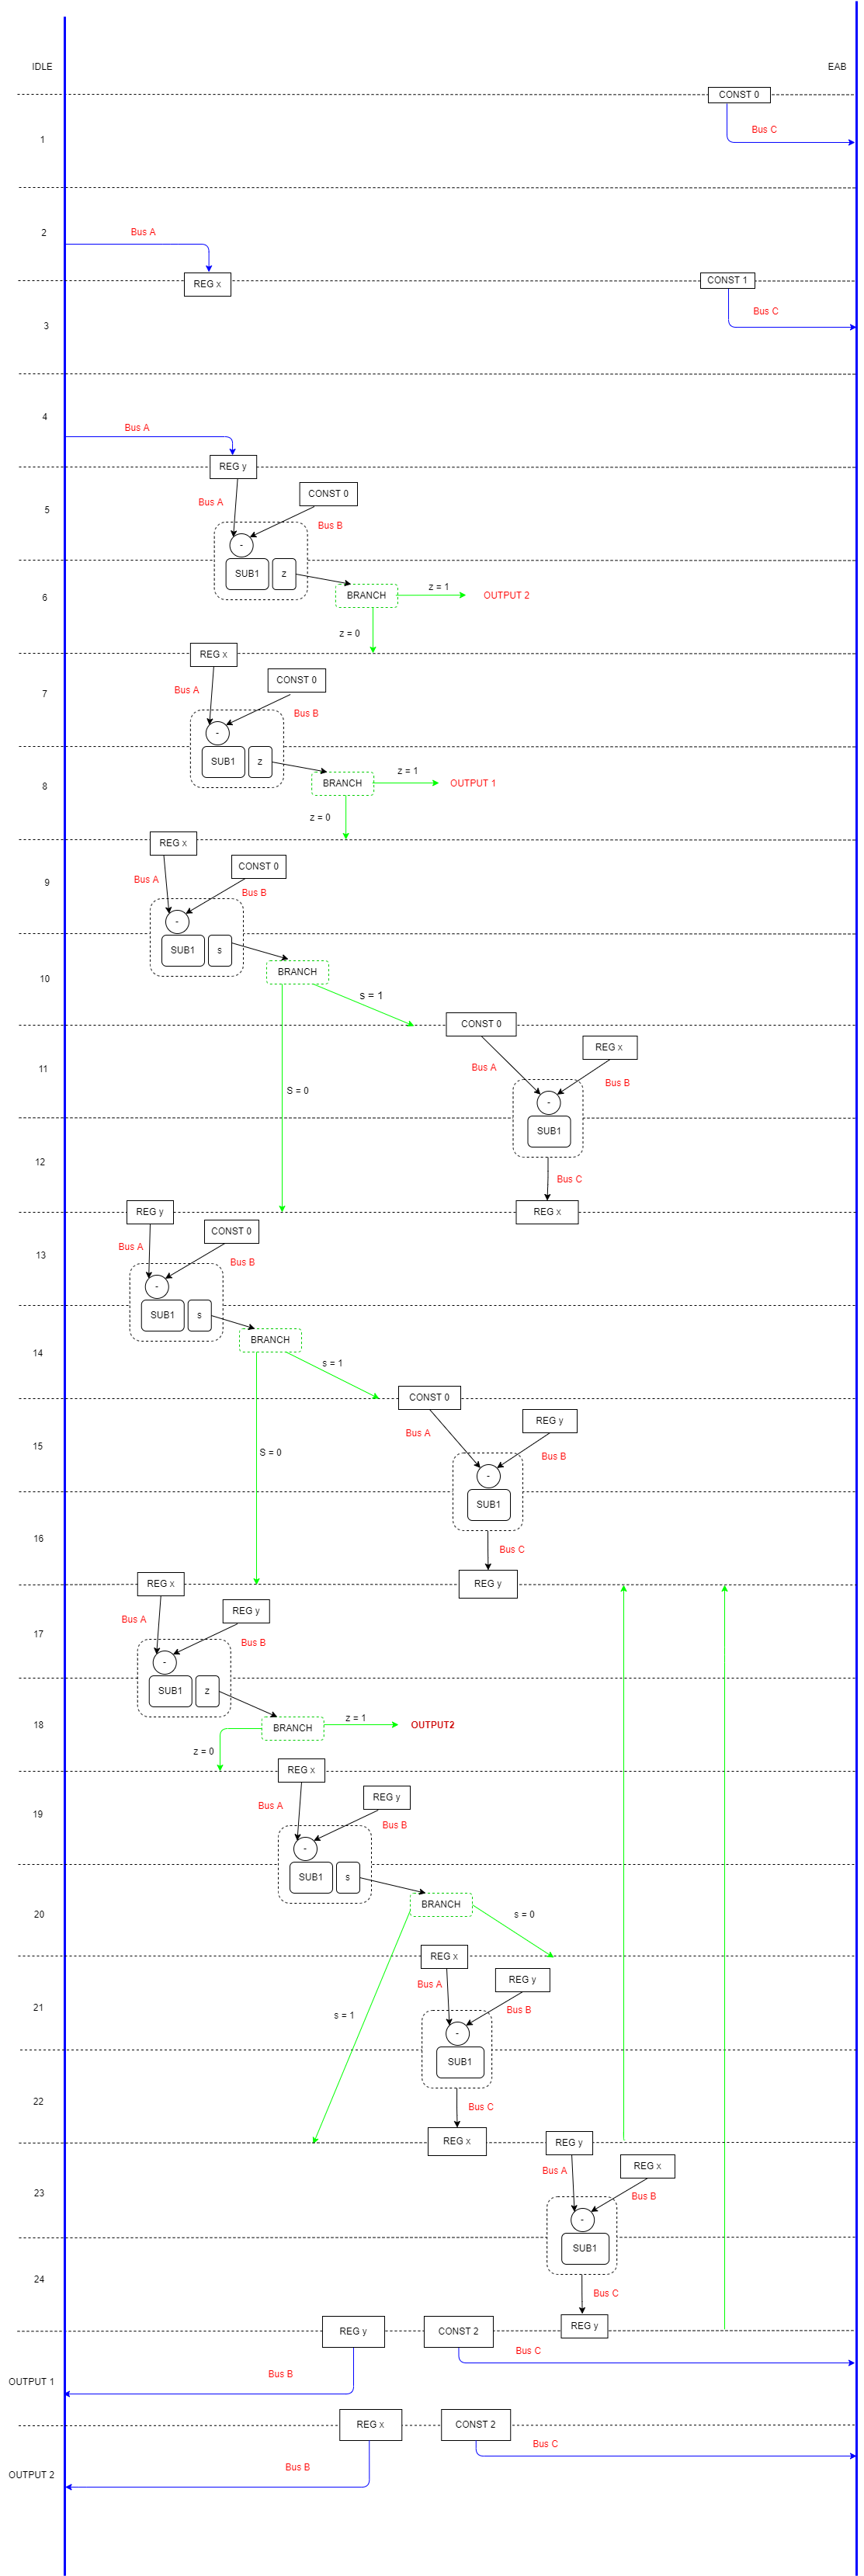
\includegraphics[width=0.5\textwidth]{images/Datenflussgraph.png}
  \caption[Datenflussgraph]{Datenflussgraph}
  \label{fig:datenflussgraph}
\end{figure}

\section{DATENFLUSSGRAPH}
Das in Abbildung 3.1 dargestellte Datenflußdiagramm des Algorithmus ist in vier Hauptteile unterteilt. Die Zustände 1-4 dienen der Initialisierung der Eingabedaten in den Registern. Die Zustände 5-16 dienen dazu, die Eingabedaten so zu verarbeiten, dass sie die Bedingungen des dritten Teils des Algorithmus erfüllen. Die Zustände 17-24 sind für den dritten Teil, den euklidischen Algorithmus. Dieser Teil dient der Berechnung des größten gemeinsamen Teilers der beiden Eingabedaten. Die Zustände OUTPUT1 und OUTPUT2 sind der vierte Teil, der dazu dient, das Endergebnis in die Register zu schreiben.

\vspace{\baselineskip}

\noindent Das Schreiben in den Speicher dauert einen Takt. Das Lesen von Daten muss nach dem Schreiben in den Speicher erfolgen. Daher darf das Schreiben von Daten in den Speicher und das Lesen von Registern aus dem Speicher nicht im selben Takt erfolgen. Bei den ersten beiden Beurteilungen des Algorithmus muss nur der Eingangswert mit 0 verglichen werden. Daher ist in diesem Prozess keine Änderung des Speichers erforderlich. Beim Euklidischen Algorithmus müssen die Werte in den Registern überschrieben werden. Die Werte in den Registern werden zur Berechnung über den Bus im vorherigen Takt an die Subtraktion gesendet. Dann wird er zum letzten Takt in das entsprechende Register transportiert, um die ursprünglichen Daten zu überschreiben. Es ist somit nicht notwendig, weitere temporäre Register zur Speicherung der Daten zu verwenden. Dies reduziert den Hardwareaufwand.

\vspace{\baselineskip}

\noindent Da der Algorithmus einfach ist. Die Dateneingabe und -ausgabe muss sequentiell in Taktfolge erfolgen. Es ist nicht möglich, durch parallele Berechnungen Zeit zu sparen. Daher besteht die einzige Möglichkeit, diesen Entwurf zu vereinfachen, in der Reduzierung des Hardwareaufwands. 

\section{DATENPFADARCHITEKTUR}

Zur Realisierung des Entwurfs werden zwei 32-Bit-Register zur Speicherung der Eingangsdaten und Zwischenwerte verwendet. Drei Konstantenregister werden auch als Indizes für das Lesen und Schreiben in den Speicher verwendet. Sie sind über den Bus C mit dem Adress-Port des Speichers verbunden. Bus A verbindet die Register mit dem DOUT-Port des Speichers und initialisiert die Register. Bus B wird verwendet, um Werte in den Speicher zu schreiben, so dass das Konstantenregister 0 und die Register x und y mit Bus B verbunden sind.

\vspace{\baselineskip}

\noindent Das Datenpfaddiagramm in Abbildung 3.2 zeigt die Verbindung zwischen den verwendeten Registern und den Bussen, wenn dieser Algorithmus ausgeführt wird. Beim Bus werden Daten zwischen den Registern und dem Speicher ausgetauscht, indem diese miteinander verbunden werden. Dieser Datenpfad ermöglicht die Operationen der Register, die Initialisierung des Speichers und die Speicherung von Konstanten.

\vspace{\baselineskip}

\noindent Die Verwendung von Registern und Bussen hilft uns, den Entwurf mit einem Minimum an Hardware zu realisieren und den Algorithmus ohne zusätzliche Schaltungen zu implementieren.

\vspace{\baselineskip}
\begin{figure}[H]
  \centering
  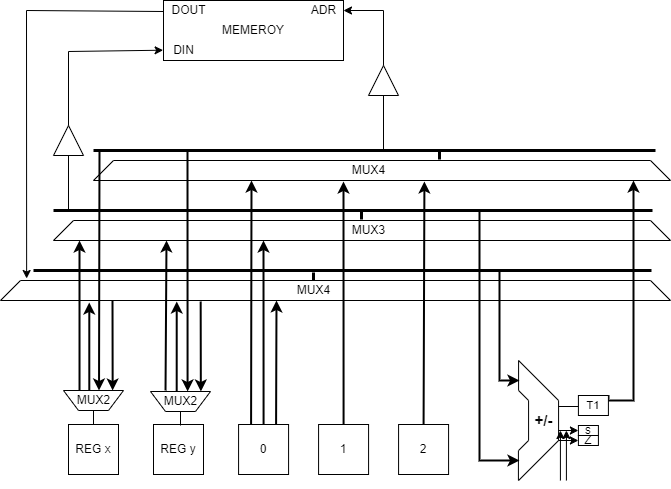
\includegraphics[width=1.0\textwidth]{images/Datenpfad.png}
  \caption[Datenpfad]{Datenpfad}
  \label{fig:datenpfad}
\end{figure}

\noindent Als Folge der oben genannten Analyse ist es möglich, das Datenpfad mit CADENCE zu erstellen. Das erstellte Diagramm ist in Abbildung 3.3 dargestellt.

\vspace{\baselineskip}

\begin{figure}[H]
  \centering
  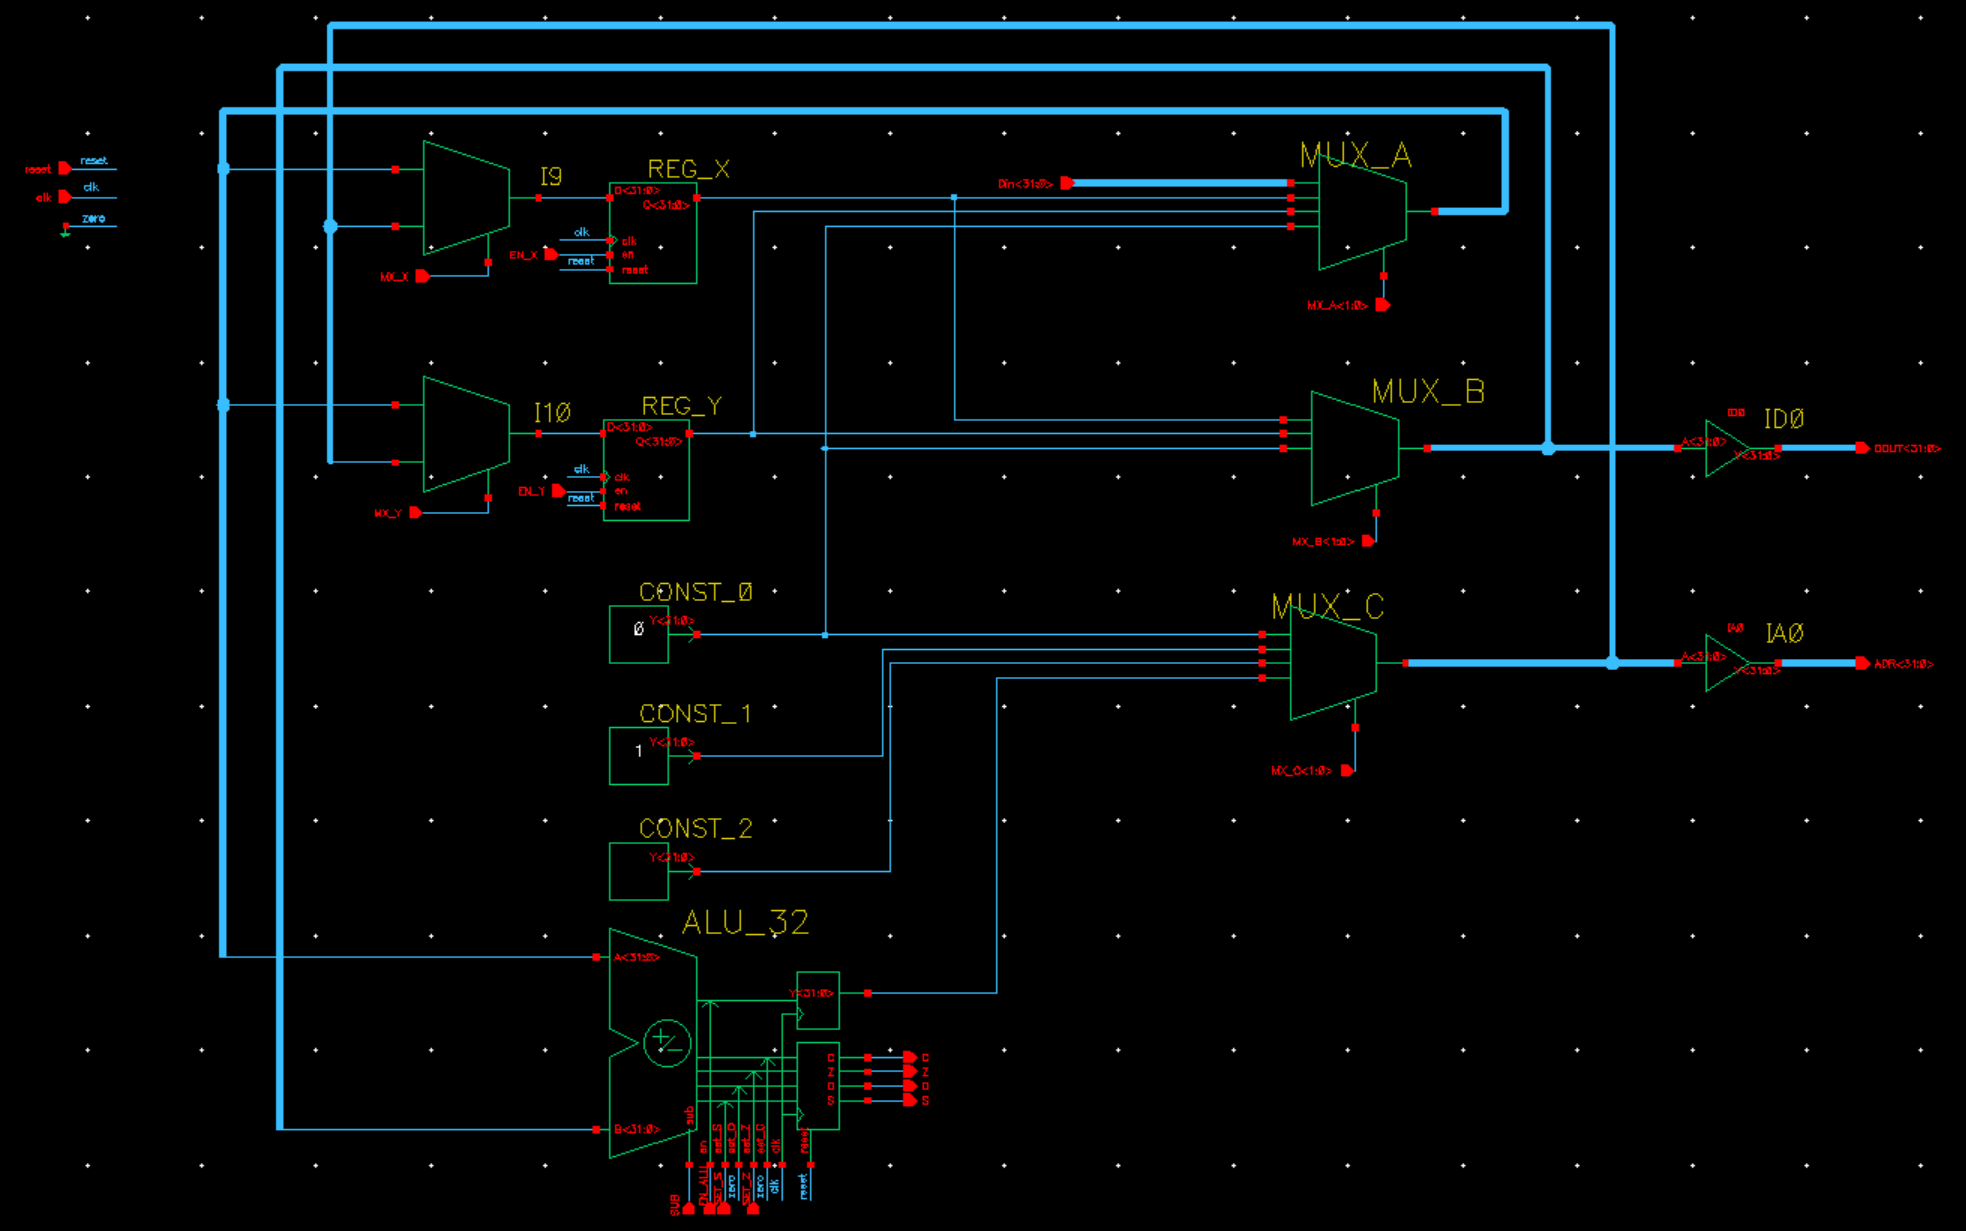
\includegraphics[width=1.0\textwidth]{images/DatapfadCADENCE.png}
  \caption[Datenpfad mit CADENCE]{Datenpfad mit CADENCE}
  \label{fig:datapfadCADENCE}
\end{figure}

\section{REGISTERTRANSFERFOLGE}

Die Registertransferfolge beschreibt die Schritte, die bei der Ausführung des Algorithmus durch den Computer durchgeführt werden müssen. Die Beschreibung wird aus Datenflussdiagrammen und Datenpfaden abgeleitet, damit die gewünschten Ergebnisse des Algorithmus erzielt werden können.

\vspace{\baselineskip}

\noindent Die Zustände der Registertransferfolge im Datenflussdiagramm sind in Abbildung 3.4 dargestellt. Dazu gehören die Zustände 1-2 und 5-6 zur Initialisierung der Eingabedaten, die Zustände 3-4 und 7-16 zur Verarbeitung der Eingabedaten, die Zustände 17-24 für den euklidischen Algorithmus und die Ausgangszustände OUTPUT1 und OUTPUT2 zum Schreiben der Ergebnisse.

\vspace{\baselineskip}

\noindent Die Verzweigung der Registertransferfolge basiert auf die Beurteilungen von Zero-Flags und Negative-Flags. Die Zero-Flags werden verwendet, um zu prüfen, ob der Algorithmus die Ausgangsbedingungen erfüllt. Ist das Flag auf 0 gesetzt, d.h. z = 0, dann sind die beiden zu vergleichenden Werte nicht gleich und der Algorithmus sollte fortgesetzt werden; ist das Flag auf 1 gesetzt, d.h. z = 1, dann sind die beiden zu vergleichenden Werte gleich und das Ergebnis sollte an dieser Stelle ausgegeben werden. Die Verzweigung mit Negative-Flags wird verwendet, um die Daten im Algorithmus zu verarbeiten. Wird das Flag auf 0 gesetzt, d.h. s = 0, bedeutet dies, dass der über Bus A transportierte Wert kleiner ist als der über Bus B transportierte Wert. Wird das Flag auf 1 gesetzt, d.h. s = 1, bedeutet dies, dass der über Bus A transportierte Wert größer oder gleich dem über Bus B transportierten Wert ist. Der Algorithmus führt die entsprechende Operation auf der Grundlage des Zustands des Negative-Flags durch.

\vspace{\baselineskip}

\noindent Wenn der Algorithmus Ergebnisse ausgibt, kehrt er in den Zustand IDLE zurück und wartet auf neue Eingaben. Insgesamt erfüllt der Algorithmus die Aufgabe mit diesem Entwurf.

\begin{figure}[H]
  \centering
  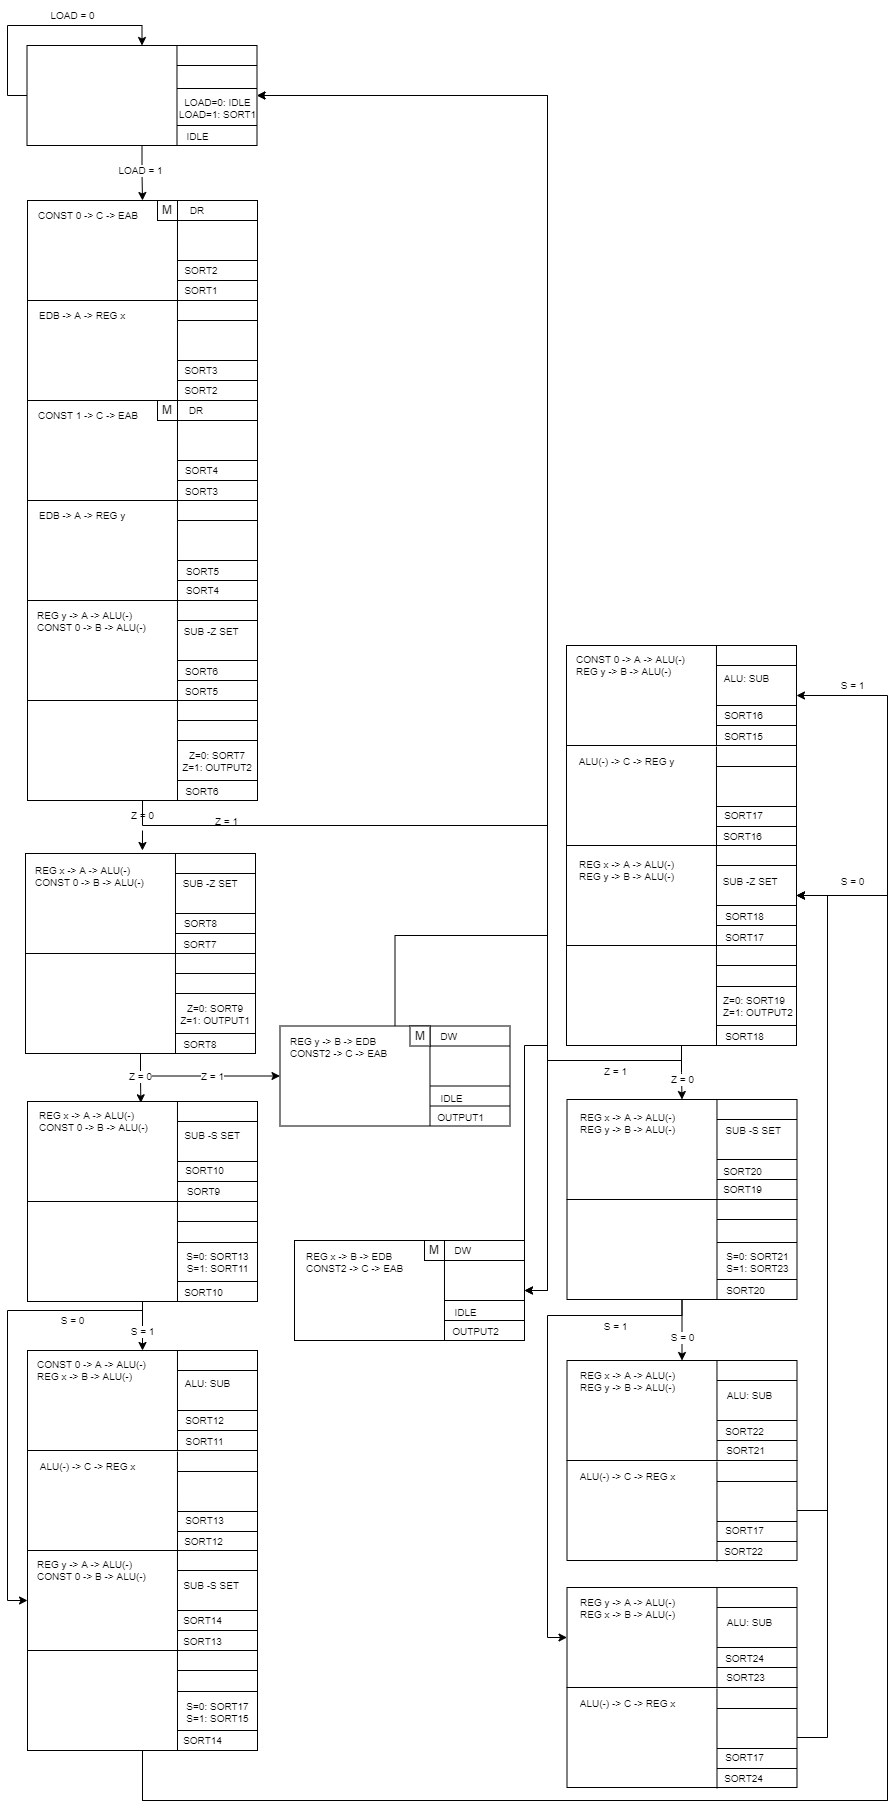
\includegraphics[width=0.7\textwidth]{images/Registertransferfolge.png}
  \caption[Registertransferfolge]{Registertransferfolge}
  \label{fig:Registertransferfolge}
\end{figure}

\section{ZUSTANDSÜBERGÄNGE}

Abbildung 3.5 zeigt den endlichen Automaten für FSM-Zustandsübergänge. Das Zustandsdiagramm ergibt sich aus der in Abbildung 3.4 dargestellten Registertransferfolge. Es zeigt deutlich die Zustandsübergänge des Algorithmus.

\begin{figure}[H]
  \centering
  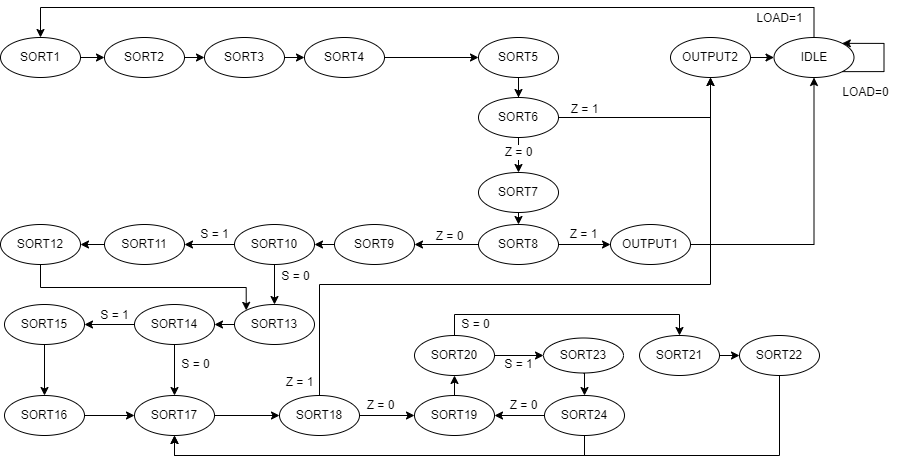
\includegraphics[width=1.0\textwidth]{images/Zustandsgraph.png}
  \caption[Zustandsgraph]{Zustandsgraph}
  \label{fig:Zustandsgraph}
\end{figure}

\noindent Die Zustandsübergangstabelle in Tabelle 3.1 zeigt die möglichen Zustandsübergänge des in Abbildung 3.5 dargestellten endlichen Zustandsautomaten. Diese Tabelle zeigt die Kombination aus dem aktuellen Zustand und dem Flag für den nächsten Zustandsübergang. Der aktuelle Zustand wird durch die Bits x4-x0 dargestellt. Der Folgezustand wird durch die Bits y4-y0 dargestellt. Die Flags in der Tabelle, die die Zustandsübergänge beeinflussen, sind die Vergleichsoperationsflags NEGATIVE und ZERO und das Datenladeflag LOAD.

\noindent Zustandsbits werden zur Steuerung eines endlichen Zustandsautomaten verwendet. Wenn bestimmte Bedingungen erfüllt sind, werden die Zustandsbits erneuert. Der Automat überführt dann in den nächsten Zustand. Der endliche Automat besteht aus 26 Zuständen. Die nicht verwendeten Zustände sind als UNUSED markiert. Die Verwendung eines endlichen Automaten ermöglicht, dass der Algorithmus Schritt für Schritt ausgeführt wird und wie erwartet funktioniert.


\begin{table}[H]
% \centering
\caption{Zustandsübergangstabelle}
\resizebox{\textwidth}{!}{
\begin{tabular}{|cccccc|ccc|cccccc|}
  \hline
  \multicolumn{6}{|c|}{Zustand}                                                                                                             & \multicolumn{3}{c|}{Flags}                                       & \multicolumn{6}{c|}{Folgezustand}                                                                                                         \\ \hline
  \multicolumn{1}{|c|}{Name}   & \multicolumn{1}{c|}{x4} & \multicolumn{1}{c|}{x3} & \multicolumn{1}{c|}{x2} & \multicolumn{1}{c|}{x1} & x0 & \multicolumn{1}{c|}{load} & \multicolumn{1}{c|}{negative} & zero & \multicolumn{1}{c|}{Name}    & \multicolumn{1}{c|}{y4} & \multicolumn{1}{c|}{y3} & \multicolumn{1}{c|}{y2} & \multicolumn{1}{c|}{y1} & y0 \\ \hline\hline
  \multicolumn{1}{|c|}{IDLE}   & \multicolumn{1}{c|}{0}  & \multicolumn{1}{c|}{0}  & \multicolumn{1}{c|}{0}  & \multicolumn{1}{c|}{0}  & 0  & \multicolumn{1}{c|}{0}    & \multicolumn{1}{c|}{-}        & -    & \multicolumn{1}{c|}{IDLE}    & \multicolumn{1}{c|}{0}  & \multicolumn{1}{c|}{0}  & \multicolumn{1}{c|}{0}  & \multicolumn{1}{c|}{0}  & 0  \\ \hline
  \multicolumn{1}{|c|}{IDLE}   & \multicolumn{1}{c|}{0}  & \multicolumn{1}{c|}{0}  & \multicolumn{1}{c|}{0}  & \multicolumn{1}{c|}{0}  & 0  & \multicolumn{1}{c|}{1}    & \multicolumn{1}{c|}{-}        & -    & \multicolumn{1}{c|}{SORT1}   & \multicolumn{1}{c|}{0}  & \multicolumn{1}{c|}{0}  & \multicolumn{1}{c|}{0}  & \multicolumn{1}{c|}{0}  & 1  \\ \hline
  \multicolumn{1}{|c|}{SORT1}  & \multicolumn{1}{c|}{0}  & \multicolumn{1}{c|}{0}  & \multicolumn{1}{c|}{0}  & \multicolumn{1}{c|}{0}  & 1  & \multicolumn{1}{c|}{-}    & \multicolumn{1}{c|}{-}        & -    & \multicolumn{1}{c|}{SORT2}   & \multicolumn{1}{c|}{0}  & \multicolumn{1}{c|}{0}  & \multicolumn{1}{c|}{0}  & \multicolumn{1}{c|}{1}  & 0  \\ \hline
  \multicolumn{1}{|c|}{SORT2}  & \multicolumn{1}{c|}{0}  & \multicolumn{1}{c|}{0}  & \multicolumn{1}{c|}{0}  & \multicolumn{1}{c|}{1}  & 0  & \multicolumn{1}{c|}{-}    & \multicolumn{1}{c|}{-}        & -    & \multicolumn{1}{c|}{SORT3}   & \multicolumn{1}{c|}{0}  & \multicolumn{1}{c|}{0}  & \multicolumn{1}{c|}{0}  & \multicolumn{1}{c|}{1}  & 1  \\ \hline
  \multicolumn{1}{|c|}{SORT3}  & \multicolumn{1}{c|}{0}  & \multicolumn{1}{c|}{0}  & \multicolumn{1}{c|}{0}  & \multicolumn{1}{c|}{1}  & 1  & \multicolumn{1}{c|}{-}    & \multicolumn{1}{c|}{-}        & -    & \multicolumn{1}{c|}{SORT4}   & \multicolumn{1}{c|}{0}  & \multicolumn{1}{c|}{0}  & \multicolumn{1}{c|}{1}  & \multicolumn{1}{c|}{0}  & 0  \\ \hline
  \multicolumn{1}{|c|}{SORT4}  & \multicolumn{1}{c|}{0}  & \multicolumn{1}{c|}{0}  & \multicolumn{1}{c|}{1}  & \multicolumn{1}{c|}{0}  & 0  & \multicolumn{1}{c|}{-}    & \multicolumn{1}{c|}{-}        & -    & \multicolumn{1}{c|}{SORT5}   & \multicolumn{1}{c|}{0}  & \multicolumn{1}{c|}{0}  & \multicolumn{1}{c|}{1}  & \multicolumn{1}{c|}{0}  & 1  \\ \hline
  \multicolumn{1}{|c|}{SORT5}  & \multicolumn{1}{c|}{0}  & \multicolumn{1}{c|}{0}  & \multicolumn{1}{c|}{1}  & \multicolumn{1}{c|}{0}  & 1  & \multicolumn{1}{c|}{-}    & \multicolumn{1}{c|}{-}        & -    & \multicolumn{1}{c|}{SORT6}   & \multicolumn{1}{c|}{0}  & \multicolumn{1}{c|}{0}  & \multicolumn{1}{c|}{1}  & \multicolumn{1}{c|}{1}  & 0  \\ \hline
  \multicolumn{1}{|c|}{SORT6}  & \multicolumn{1}{c|}{0}  & \multicolumn{1}{c|}{0}  & \multicolumn{1}{c|}{1}  & \multicolumn{1}{c|}{1}  & 0  & \multicolumn{1}{c|}{-}    & \multicolumn{1}{c|}{-}        & 0    & \multicolumn{1}{c|}{SORT7}   & \multicolumn{1}{c|}{0}  & \multicolumn{1}{c|}{0}  & \multicolumn{1}{c|}{1}  & \multicolumn{1}{c|}{1}  & 1  \\ \hline
  \multicolumn{1}{|c|}{SORT6}  & \multicolumn{1}{c|}{0}  & \multicolumn{1}{c|}{0}  & \multicolumn{1}{c|}{1}  & \multicolumn{1}{c|}{1}  & 0  & \multicolumn{1}{c|}{-}    & \multicolumn{1}{c|}{-}        & 1    & \multicolumn{1}{c|}{OUTPUT2} & \multicolumn{1}{c|}{1}  & \multicolumn{1}{c|}{1}  & \multicolumn{1}{c|}{0}  & \multicolumn{1}{c|}{1}  & 0  \\ \hline
  \multicolumn{1}{|c|}{SORT7}  & \multicolumn{1}{c|}{0}  & \multicolumn{1}{c|}{0}  & \multicolumn{1}{c|}{1}  & \multicolumn{1}{c|}{1}  & 1  & \multicolumn{1}{c|}{-}    & \multicolumn{1}{c|}{-}        & -    & \multicolumn{1}{c|}{SORT8}   & \multicolumn{1}{c|}{0}  & \multicolumn{1}{c|}{1}  & \multicolumn{1}{c|}{0}  & \multicolumn{1}{c|}{0}  & 0  \\ \hline
  \multicolumn{1}{|c|}{SORT8}  & \multicolumn{1}{c|}{0}  & \multicolumn{1}{c|}{1}  & \multicolumn{1}{c|}{0}  & \multicolumn{1}{c|}{0}  & 0  & \multicolumn{1}{c|}{-}    & \multicolumn{1}{c|}{-}        & 0    & \multicolumn{1}{c|}{SORT9}   & \multicolumn{1}{c|}{0}  & \multicolumn{1}{c|}{1}  & \multicolumn{1}{c|}{0}  & \multicolumn{1}{c|}{0}  & 1  \\ \hline
  \multicolumn{1}{|c|}{SORT8}  & \multicolumn{1}{c|}{0}  & \multicolumn{1}{c|}{1}  & \multicolumn{1}{c|}{0}  & \multicolumn{1}{c|}{0}  & 0  & \multicolumn{1}{c|}{-}    & \multicolumn{1}{c|}{-}        & 1    & \multicolumn{1}{c|}{OUTPUT1} & \multicolumn{1}{c|}{1}  & \multicolumn{1}{c|}{1}  & \multicolumn{1}{c|}{0}  & \multicolumn{1}{c|}{0}  & 1  \\ \hline
  \multicolumn{1}{|c|}{SORT9}  & \multicolumn{1}{c|}{0}  & \multicolumn{1}{c|}{1}  & \multicolumn{1}{c|}{0}  & \multicolumn{1}{c|}{0}  & 1  & \multicolumn{1}{c|}{-}    & \multicolumn{1}{c|}{-}        & -    & \multicolumn{1}{c|}{SORT10}  & \multicolumn{1}{c|}{0}  & \multicolumn{1}{c|}{1}  & \multicolumn{1}{c|}{0}  & \multicolumn{1}{c|}{1}  & 0  \\ \hline
  \multicolumn{1}{|c|}{SORT10} & \multicolumn{1}{c|}{0}  & \multicolumn{1}{c|}{1}  & \multicolumn{1}{c|}{0}  & \multicolumn{1}{c|}{1}  & 0  & \multicolumn{1}{c|}{-}    & \multicolumn{1}{c|}{0}        & -    & \multicolumn{1}{c|}{SORT13}  & \multicolumn{1}{c|}{0}  & \multicolumn{1}{c|}{1}  & \multicolumn{1}{c|}{1}  & \multicolumn{1}{c|}{0}  & 1  \\ \hline
  \multicolumn{1}{|c|}{SORT10} & \multicolumn{1}{c|}{0}  & \multicolumn{1}{c|}{1}  & \multicolumn{1}{c|}{0}  & \multicolumn{1}{c|}{1}  & 0  & \multicolumn{1}{c|}{-}    & \multicolumn{1}{c|}{1}        & -    & \multicolumn{1}{c|}{SORT11}  & \multicolumn{1}{c|}{0}  & \multicolumn{1}{c|}{1}  & \multicolumn{1}{c|}{0}  & \multicolumn{1}{c|}{1}  & 1  \\ \hline
  \multicolumn{1}{|c|}{SORT11} & \multicolumn{1}{c|}{0}  & \multicolumn{1}{c|}{1}  & \multicolumn{1}{c|}{0}  & \multicolumn{1}{c|}{1}  & 1  & \multicolumn{1}{c|}{-}    & \multicolumn{1}{c|}{-}        & -    & \multicolumn{1}{c|}{SORT12}  & \multicolumn{1}{c|}{0}  & \multicolumn{1}{c|}{1}  & \multicolumn{1}{c|}{1}  & \multicolumn{1}{c|}{0}  & 0  \\ \hline
  \multicolumn{1}{|c|}{SORT12} & \multicolumn{1}{c|}{0}  & \multicolumn{1}{c|}{1}  & \multicolumn{1}{c|}{1}  & \multicolumn{1}{c|}{0}  & 0  & \multicolumn{1}{c|}{-}    & \multicolumn{1}{c|}{-}        & -    & \multicolumn{1}{c|}{SORT13}  & \multicolumn{1}{c|}{0}  & \multicolumn{1}{c|}{1}  & \multicolumn{1}{c|}{1}  & \multicolumn{1}{c|}{0}  & 1  \\ \hline
  \multicolumn{1}{|c|}{SORT13}  & \multicolumn{1}{c|}{0}  & \multicolumn{1}{c|}{1}  & \multicolumn{1}{c|}{1}  & \multicolumn{1}{c|}{0}  & 1  & \multicolumn{1}{c|}{-}    & \multicolumn{1}{c|}{-}        & -    & \multicolumn{1}{c|}{SORT14}  & \multicolumn{1}{c|}{0}  & \multicolumn{1}{c|}{1}  & \multicolumn{1}{c|}{1}  & \multicolumn{1}{c|}{1}  & 0  \\ \hline
\multicolumn{1}{|c|}{SORT14}  & \multicolumn{1}{c|}{0}  & \multicolumn{1}{c|}{1}  & \multicolumn{1}{c|}{1}  & \multicolumn{1}{c|}{1}  & 0  & \multicolumn{1}{c|}{-}    & \multicolumn{1}{c|}{0}        & -    & \multicolumn{1}{c|}{SORT17}  & \multicolumn{1}{c|}{1}  & \multicolumn{1}{c|}{0}  & \multicolumn{1}{c|}{0}  & \multicolumn{1}{c|}{0}  & 1  \\ \hline
\multicolumn{1}{|c|}{SORT14}  & \multicolumn{1}{c|}{0}  & \multicolumn{1}{c|}{1}  & \multicolumn{1}{c|}{1}  & \multicolumn{1}{c|}{1}  & 0  & \multicolumn{1}{c|}{-}    & \multicolumn{1}{c|}{1}        & -    & \multicolumn{1}{c|}{SORT15}  & \multicolumn{1}{c|}{0}  & \multicolumn{1}{c|}{1}  & \multicolumn{1}{c|}{1}  & \multicolumn{1}{c|}{1}  & 1  \\ \hline
\multicolumn{1}{|c|}{SORT15}  & \multicolumn{1}{c|}{0}  & \multicolumn{1}{c|}{1}  & \multicolumn{1}{c|}{1}  & \multicolumn{1}{c|}{1}  & 1  & \multicolumn{1}{c|}{-}    & \multicolumn{1}{c|}{-}        & -    & \multicolumn{1}{c|}{SORT16}  & \multicolumn{1}{c|}{1}  & \multicolumn{1}{c|}{0}  & \multicolumn{1}{c|}{0}  & \multicolumn{1}{c|}{0}  & 0  \\ \hline
\multicolumn{1}{|c|}{SORT16}  & \multicolumn{1}{c|}{1}  & \multicolumn{1}{c|}{0}  & \multicolumn{1}{c|}{0}  & \multicolumn{1}{c|}{0}  & 0  & \multicolumn{1}{c|}{-}    & \multicolumn{1}{c|}{-}        & -    & \multicolumn{1}{c|}{SORT17}  & \multicolumn{1}{c|}{1}  & \multicolumn{1}{c|}{0}  & \multicolumn{1}{c|}{0}  & \multicolumn{1}{c|}{0}  & 1  \\ \hline
\multicolumn{1}{|c|}{SORT17}  & \multicolumn{1}{c|}{1}  & \multicolumn{1}{c|}{0}  & \multicolumn{1}{c|}{0}  & \multicolumn{1}{c|}{0}  & 1  & \multicolumn{1}{c|}{-}    & \multicolumn{1}{c|}{-}        & -    & \multicolumn{1}{c|}{SORT18}  & \multicolumn{1}{c|}{1}  & \multicolumn{1}{c|}{0}  & \multicolumn{1}{c|}{0}  & \multicolumn{1}{c|}{1}  & 0  \\ \hline
\multicolumn{1}{|c|}{SORT18}  & \multicolumn{1}{c|}{1}  & \multicolumn{1}{c|}{0}  & \multicolumn{1}{c|}{0}  & \multicolumn{1}{c|}{1}  & 0  & \multicolumn{1}{c|}{-}    & \multicolumn{1}{c|}{-}        & 0    & \multicolumn{1}{c|}{SORT19}  & \multicolumn{1}{c|}{1}  & \multicolumn{1}{c|}{0}  & \multicolumn{1}{c|}{0}  & \multicolumn{1}{c|}{1}  & 1  \\ \hline
\multicolumn{1}{|c|}{SORT18}  & \multicolumn{1}{c|}{1}  & \multicolumn{1}{c|}{0}  & \multicolumn{1}{c|}{0}  & \multicolumn{1}{c|}{1}  & 0  & \multicolumn{1}{c|}{-}    & \multicolumn{1}{c|}{-}        & 1    & \multicolumn{1}{c|}{OUTPUT2} & \multicolumn{1}{c|}{1}  & \multicolumn{1}{c|}{1}  & \multicolumn{1}{c|}{0}  & \multicolumn{1}{c|}{1}  & 0  \\ \hline
\multicolumn{1}{|c|}{SORT19}  & \multicolumn{1}{c|}{1}  & \multicolumn{1}{c|}{0}  & \multicolumn{1}{c|}{0}  & \multicolumn{1}{c|}{1}  & 1  & \multicolumn{1}{c|}{-}    & \multicolumn{1}{c|}{-}        & -    & \multicolumn{1}{c|}{SORT20}  & \multicolumn{1}{c|}{1}  & \multicolumn{1}{c|}{0}  & \multicolumn{1}{c|}{1}  & \multicolumn{1}{c|}{0}  & 0  \\ \hline
\multicolumn{1}{|c|}{SORT20}  & \multicolumn{1}{c|}{1}  & \multicolumn{1}{c|}{0}  & \multicolumn{1}{c|}{1}  & \multicolumn{1}{c|}{0}  & 0  & \multicolumn{1}{c|}{-}    & \multicolumn{1}{c|}{0}        & -    & \multicolumn{1}{c|}{SORT21}  & \multicolumn{1}{c|}{1}  & \multicolumn{1}{c|}{0}  & \multicolumn{1}{c|}{1}  & \multicolumn{1}{c|}{0}  & 1  \\ \hline
\multicolumn{1}{|c|}{SORT20}  & \multicolumn{1}{c|}{1}  & \multicolumn{1}{c|}{0}  & \multicolumn{1}{c|}{1}  & \multicolumn{1}{c|}{0}  & 0  & \multicolumn{1}{c|}{-}    & \multicolumn{1}{c|}{1}        & -    & \multicolumn{1}{c|}{SORT23}  & \multicolumn{1}{c|}{1}  & \multicolumn{1}{c|}{0}  & \multicolumn{1}{c|}{1}  & \multicolumn{1}{c|}{1}  & 1  \\ \hline
\multicolumn{1}{|c|}{SORT21}  & \multicolumn{1}{c|}{1}  & \multicolumn{1}{c|}{0}  & \multicolumn{1}{c|}{1}  & \multicolumn{1}{c|}{0}  & 1  & \multicolumn{1}{c|}{-}    & \multicolumn{1}{c|}{-}        & -    & \multicolumn{1}{c|}{SORT22}  & \multicolumn{1}{c|}{1}  & \multicolumn{1}{c|}{0}  & \multicolumn{1}{c|}{1}  & \multicolumn{1}{c|}{1}  & 0  \\ \hline
\multicolumn{1}{|c|}{SORT22}  & \multicolumn{1}{c|}{1}  & \multicolumn{1}{c|}{0}  & \multicolumn{1}{c|}{1}  & \multicolumn{1}{c|}{1}  & 0  & \multicolumn{1}{c|}{-}    & \multicolumn{1}{c|}{-}        & -    & \multicolumn{1}{c|}{SORT17}  & \multicolumn{1}{c|}{1}  & \multicolumn{1}{c|}{0}  & \multicolumn{1}{c|}{0}  & \multicolumn{1}{c|}{0}  & 1  \\ \hline
\multicolumn{1}{|c|}{SORT23}  & \multicolumn{1}{c|}{1}  & \multicolumn{1}{c|}{0}  & \multicolumn{1}{c|}{1}  & \multicolumn{1}{c|}{1}  & 1  & \multicolumn{1}{c|}{-}    & \multicolumn{1}{c|}{-}        & -    & \multicolumn{1}{c|}{SORT24}  & \multicolumn{1}{c|}{1}  & \multicolumn{1}{c|}{1}  & \multicolumn{1}{c|}{0}  & \multicolumn{1}{c|}{0}  & 0  \\ \hline
\multicolumn{1}{|c|}{SORT24}  & \multicolumn{1}{c|}{1}  & \multicolumn{1}{c|}{1}  & \multicolumn{1}{c|}{0}  & \multicolumn{1}{c|}{0}  & 0  & \multicolumn{1}{c|}{-}    & \multicolumn{1}{c|}{-}        & -    & \multicolumn{1}{c|}{SORT17}  & \multicolumn{1}{c|}{1}  & \multicolumn{1}{c|}{0}  & \multicolumn{1}{c|}{0}  & \multicolumn{1}{c|}{0}  & 1  \\ \hline
\multicolumn{1}{|c|}{OUTPUT1} & \multicolumn{1}{c|}{1}  & \multicolumn{1}{c|}{1}  & \multicolumn{1}{c|}{0}  & \multicolumn{1}{c|}{0}  & 1  & \multicolumn{1}{c|}{-}    & \multicolumn{1}{c|}{-}        & -    & \multicolumn{1}{c|}{IDLE}    & \multicolumn{1}{c|}{0}  & \multicolumn{1}{c|}{0}  & \multicolumn{1}{c|}{0}  & \multicolumn{1}{c|}{0}  & 0  \\ \hline
\multicolumn{1}{|c|}{OUTPUT2} & \multicolumn{1}{c|}{1}  & \multicolumn{1}{c|}{1}  & \multicolumn{1}{c|}{0}  & \multicolumn{1}{c|}{1}  & 0  & \multicolumn{1}{c|}{-}    & \multicolumn{1}{c|}{-}        & -    & \multicolumn{1}{c|}{IDLE}    & \multicolumn{1}{c|}{0}  & \multicolumn{1}{c|}{0}  & \multicolumn{1}{c|}{0}  & \multicolumn{1}{c|}{0}  & 0  \\ \hline
\multicolumn{1}{|c|}{UNUSED1} & \multicolumn{1}{c|}{1}  & \multicolumn{1}{c|}{1}  & \multicolumn{1}{c|}{0}  & \multicolumn{1}{c|}{1}  & 1  & \multicolumn{1}{c|}{-}    & \multicolumn{1}{c|}{-}        & -    & \multicolumn{1}{c|}{IDLE}    & \multicolumn{1}{c|}{0}  & \multicolumn{1}{c|}{0}  & \multicolumn{1}{c|}{0}  & \multicolumn{1}{c|}{0}  & 0  \\ \hline
\multicolumn{1}{|c|}{UNUSED2} & \multicolumn{1}{c|}{1}  & \multicolumn{1}{c|}{1}  & \multicolumn{1}{c|}{1}  & \multicolumn{1}{c|}{0}  & 0  & \multicolumn{1}{c|}{-}    & \multicolumn{1}{c|}{-}        & -    & \multicolumn{1}{c|}{IDLE}    & \multicolumn{1}{c|}{0}  & \multicolumn{1}{c|}{0}  & \multicolumn{1}{c|}{0}  & \multicolumn{1}{c|}{0}  & 0  \\ \hline
\multicolumn{1}{|c|}{UNUSED3} & \multicolumn{1}{c|}{1}  & \multicolumn{1}{c|}{1}  & \multicolumn{1}{c|}{1}  & \multicolumn{1}{c|}{0}  & 1  & \multicolumn{1}{c|}{-}    & \multicolumn{1}{c|}{-}        & -    & \multicolumn{1}{c|}{IDLE}    & \multicolumn{1}{c|}{0}  & \multicolumn{1}{c|}{0}  & \multicolumn{1}{c|}{0}  & \multicolumn{1}{c|}{0}  & 0  \\ \hline
\multicolumn{1}{|c|}{UNUSED4} & \multicolumn{1}{c|}{1}  & \multicolumn{1}{c|}{1}  & \multicolumn{1}{c|}{1}  & \multicolumn{1}{c|}{1}  & 0  & \multicolumn{1}{c|}{-}    & \multicolumn{1}{c|}{-}        & -    & \multicolumn{1}{c|}{IDLE}    & \multicolumn{1}{c|}{0}  & \multicolumn{1}{c|}{0}  & \multicolumn{1}{c|}{0}  & \multicolumn{1}{c|}{0}  & 0  \\ \hline
\multicolumn{1}{|c|}{UNUSED5} & \multicolumn{1}{c|}{1}  & \multicolumn{1}{c|}{1}  & \multicolumn{1}{c|}{1}  & \multicolumn{1}{c|}{1}  & 1  & \multicolumn{1}{c|}{-}    & \multicolumn{1}{c|}{-}        & -    & \multicolumn{1}{c|}{IDLE}    & \multicolumn{1}{c|}{0}  & \multicolumn{1}{c|}{0}  & \multicolumn{1}{c|}{0}  & \multicolumn{1}{c|}{0}  & 0  \\ \hline
\end{tabular}}
\end{table}


\section{LOGIKGLEICHUNGEN}

Die vereinfachten logischen Gleichungen 3.1-3.5 erhält man durch Eingabe der Wahrheitstabelle aus Tabelle 3.1 mit LOGICFRIDAY.

\begin{equation}
y4 = x4\overline{x3} + x4\overline{x1}\overline{x0} + x3x2x1\overline{negative} + \overline{x3}x2\overline{x1x0}zero + x3\overline{x2x1x0}zero \label{3.1}
\end{equation}

\begin{equation}
  y3 = \overline{x4}x3 \overline{x2} + \overline{x3}x2x1x0 + \overline{x4}x2\overline{x1x0}zero + x4\overline{x3x2}x1\overline{x0}zero + x3x2\overline{x1} + x3x2\overline{x0}negative \label{3.2}
\end{equation}

\begin{equation}
	\begin{split}
  y2 = & x4x2\overline{x1} + x3x2\overline{x1} + \overline{x2}x1x0 + x2\overline{x1}x0 + \overline{x4x3}x2x1\overline{x0} + \overline{x4}x3\overline{x2}x1\overline{negative} + \\
       & \overline{x4}x2x1\overline{x0}negative + \overline{x4x3}x2\overline{x0zero} \label{3.3}
  \end{split}
\end{equation}

\begin{equation}
  \begin{split}
  y1 = & \overline{x4x1}x0 + \overline{x3x1}x0 + \overline{x4x3}x1\overline{x0} + \overline{x3x2}x1\overline{x0} + x4x2\overline{x1}negative + \overline{x4}x1\overline{x0}negative + \\
       & \overline{x4}x3\overline{x2x1}zero \label{3.4}
  \end{split}
\end{equation}

\begin{equation}
  y0 = x2\overline{x0} + \overline{x4}x1\overline{x0} + x4\overline{x1x0} + \overline{x3x1x0}load + \overline{x3}x1\overline{x0zero} + x3\overline{x1x0zero} \label{3.5}
\end{equation}

\section{REALISIERUNG DER FSM}

Die fünf Ausgänge (y0-y4) der logischen Gleichungen dieses Algorithmus werden aus der Kombination der Zustandsbits (x0-x4) der Eingangsvariablen und der drei Flaggenbits (LOAD, NEGOTIVE, ZERO) erstellt. Auf der Grundlage der Gleichungen 3.1-3.5 können die entsprechenden Gatterschaltungen erzeugt werden (Abbildung 3.6).

\vspace{\baselineskip}

\begin{figure}[H]
  \centering
  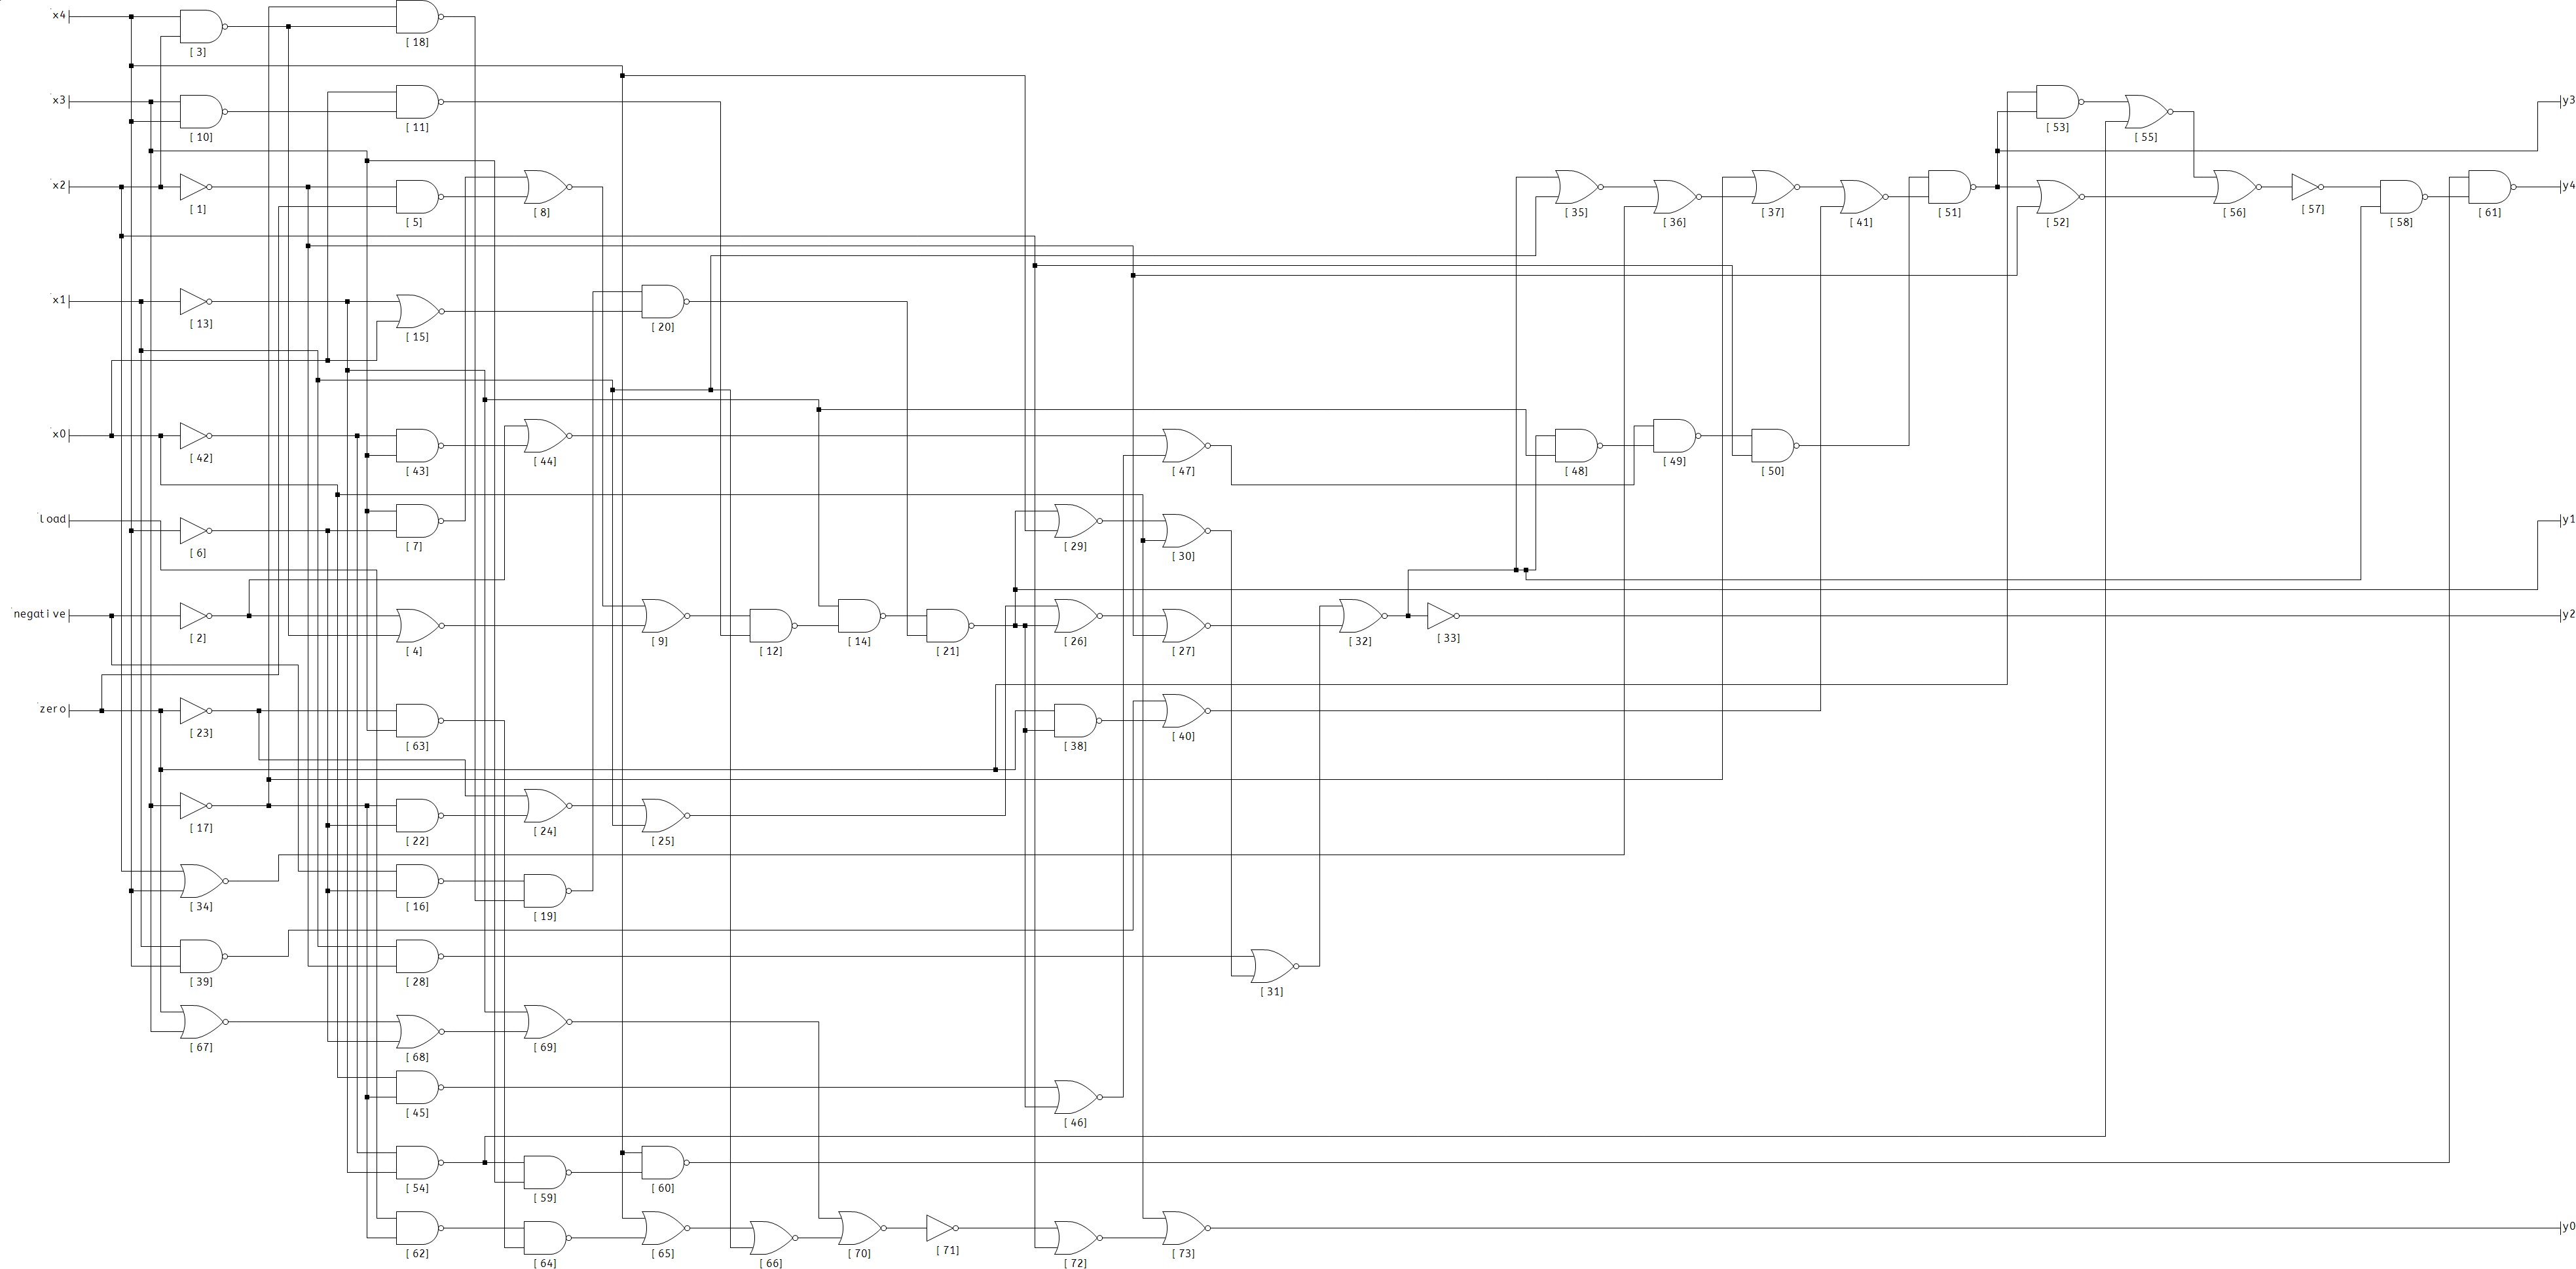
\includegraphics[width=0.9\textwidth]{images/FSM.png}
  \caption[FSM]{FSM}
  \label{fig:FSM}
\end{figure}

\section{STEUERLOGIK}

Die Steuerlogik dient zur Steuerung der Ausführung von Datenpfadbefehlen. Der Quellcode für die Steuerlogik befindet sich im Anhang. Der Code beschreibt die Funktion und die erforderlichen Befehle für jeden Zustand. Die Steuerlogik ist wichtig für die vollständige Implementierung des Algorithmus.

\section{GESAMTSCHALTUNG}

Die Gesamtschaltung besteht aus drei Teilen - FSM, Datenpfad und Logiksteuerung. Das FSM dient als Eingang für die Logiksteuerung und liefert den aktuellen Zustand des Algorithmus. Die Logiksteuerung erzeugt Steuersignale für den aktuellen Zustand und leitet sie an den Datenpfad weiter. Der Datenpfad führt die Steuersignale aus und schreibt das Ergebnis auf den Datenbus oder liest Daten vom Datenbus (EDB). Der externe Adressbus (EAB) wird zur Steuerung der Speicheradresse verwendet, von der Daten gelesen oder geschrieben werden.

\vspace{\baselineskip}

\noindent Abbildung 3.7 zeigt ein schematisches Diagramm der Gesamtschaltung, bestehend aus FSM, Datenpfad und Logiksteuerung. Alle Komponenten sind sowohl über Busse als auch über interne Busse verbunden. Die Gesamtschaltung führt den Prozess der Berechnung des größten gemeinsamen Teilers durch und kann die Daten lesen und das Ergebnis schreiben.

\begin{figure}[H]
  \centering
  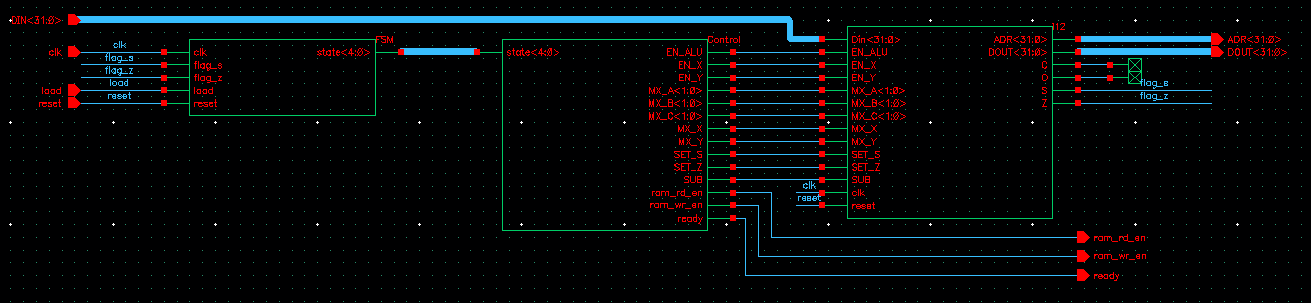
\includegraphics[width=1.0\textwidth]{images/TOP.png}
  \caption[Gesamtschaltung in CADENCE]{Gesamtschaltung in CADENCE}
  \label{fig:Gesamtschaltung}
\end{figure}

\clearpage


